\documentclass{article}
\usepackage{tikz}
\usetikzlibrary{arrows.meta,positioning,calc,shapes.geometric}
\pagestyle{empty}
\begin{document}
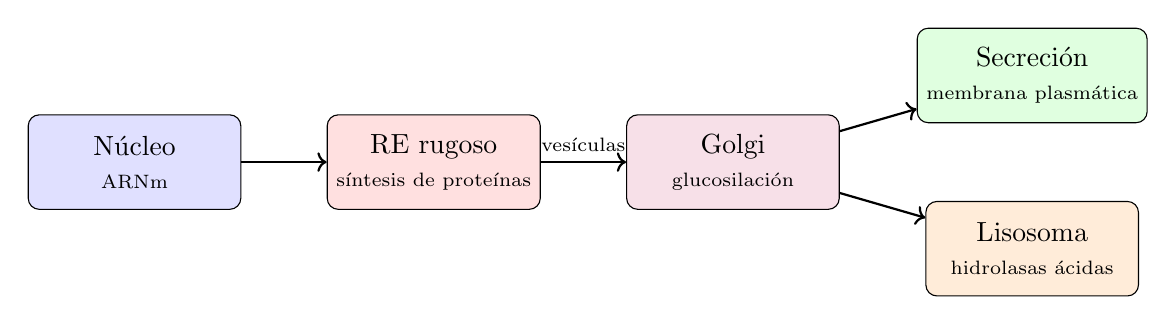
\begin{tikzpicture}
\tikzset{every node/.append style={align=center}}

\def\b#1#2#3#4{\node[draw, rounded corners, fill=#4, minimum width=2.7cm, minimum height=1.2cm, align=center] (#1) at (#2,#3) {#1};}
\node[draw, rounded corners, fill=blue!12, minimum width=2.7cm, minimum height=1.2cm, align=center] (n) at (0,0) {Núcleo\\ \scriptsize ARNm};
\node[draw, rounded corners, fill=red!12, minimum width=2.7cm, minimum height=1.2cm, align=center] (r) at (3.8,0) {RE rugoso\\ \scriptsize síntesis de proteínas};
\node[draw, rounded corners, fill=purple!12, minimum width=2.7cm, minimum height=1.2cm, align=center] (g) at (7.6,0) {Golgi\\ \scriptsize glucosilación};
\node[draw, rounded corners, fill=green!12, minimum width=2.7cm, minimum height=1.2cm, align=center] (s) at (11.4,1.1) {Secreción\\ \scriptsize membrana plasmática};
\node[draw, rounded corners, fill=orange!15, minimum width=2.7cm, minimum height=1.2cm, align=center] (l) at (11.4,-1.1) {Lisosoma\\ \scriptsize hidrolasas ácidas};
\draw[->, thick] (n) -- (r); \draw[->, thick] (r) -- node[above, font=\scriptsize] {vesículas} (g);
\draw[->, thick] (g) -- (s); \draw[->, thick] (g) -- (l);

\end{tikzpicture}
\end{document}
